\documentclass[a4paper,12pt]{report}
\usepackage{color}
\usepackage{hyperref}
\hypersetup{
    colorlinks,
    citecolor=black,
    filecolor=black,
    linkcolor=black,
    urlcolor=black
}
\setcounter{secnumdepth}{0}
\usepackage{graphicx}
\usepackage{epstopdf}
\epstopdfsetup{outdir=./}
\usepackage{amsmath}
\usepackage[table,xcdraw]{xcolor}
\usepackage{amssymb}
\usepackage{listings}
\definecolor{anti-flashwhite}{rgb}{0.95, 0.95, 0.96}
\lstset{
	language=C++,
    basicstyle=\ttfamily,
    keywordstyle=\color{blue}\ttfamily,
    stringstyle=\color{red}\ttfamily,
	commentstyle=\color{green}\ttfamily,
    morecomment=[l][\color{magenta}]{\#},
    backgroundcolor=\color{anti-flashwhite}
}
\begin{document}
\title{
\textbf{Operating Systems - II: CS3523}\\~\\
\begin{large}
\textbf{Programming Assignment - III\\~\\Implement solutions to Readers-Writers and Fair
Readers-Writers problems using Semaphores\\~\\}
\end{large}
\begin{large}
\textbf{Assignment Report}
\end{large}
}
\author{\textbf{Sagar Jain - CS17BTECH11034}\\}
\maketitle
\begin{large}
\tableofcontents
\end{large}
\newpage
\section{Program Design}
Both the algorithms i.e. \textbf{Readers-Writers} and \textbf{Fair Readers-Writers} have been implemented using Semaphores from the header \textbf{semaphore.h}. Implementation details for both the solutions is given below along with code-snippets.
\subsection{Reader-Writers}
Semaphores have been implemented using the header \textbf{\textit{semaphore.h}}
\begin{enumerate}
\item Readers-Writers is solved using the two semaphores \textit{\textbf{rw\_mutex}}, \textbf{\textit{mutex}} and an integer read\_count.
\item The semaphore \textit{\textbf{mutex}} is used to avoid race condition when accessing the variable \textit{\textbf{read\_count}}.
\item The variable \textit{\textbf{read\_count}} is used to keep a count on the number of readers, when the number of readers is $\geq 1$, then the semaphore \textbf{\textit{rw\_mutex}} makes sure that no writer can access its critical section.
\item Once the number of readers is 0, the semaphore \textit{\textbf{rw\_mutex}} is signalled which gives a chance to the writers to enter their critical section, all this is accomplished by putting conditions on the variable \textit{\textbf{read\_count}} everytime a new reader attempts to enter its critical section.
\item \textbf{Algorithm}\\\\
This is how the above can be implemented in C++.\\\\
\textbf{For Reader}:
\begin{lstlisting}
sem_wait(&mutex);
read_count++;
if (read_count == 1)
	sem_wait(&rw_mutex);
sem_post(&mutex);
// Critical Section
sem_wait(&mutex);
read_count--;
if(read_count == 0)
	sem_post(&rw_mutex);
sem_post(&mutex);
\end{lstlisting}
\textbf{For Writer}:
\begin{lstlisting}
sem_wait(&rw_mutex);
// Critical Section
sem_post(&rw_mutex);
\end{lstlisting}
\end{enumerate}
\subsection{Fair Readers-Writers}
\begin{enumerate}
\item Fair Readers-Writers is implemented using the semaphores \textbf{\textit{in}}, \textbf{\textit{out}}, \textbf{\textit{wrt}} and the integers \textbf{\textit{ctrin}}, \textbf{\textit{ctrout}}.
\item In the previous solution there exists the possibility of writer threads starving when new reader threads keep requesting to enter the critical section.
\item This problem is solved in this approach by using seperate semaphores for entry and exit and the boolean \textit{\textbf{wait}}. Once a writer thread requests for entry into the critical section, no new reader thread can enter the critical section before the writer thread finishes since the writer thread blocks the reader threads using the semaphore \textbf{\textit{in}}.
\item The reader threads are allowed to exit once the writer thread requests entry into the critical section, then through the semaphore \textbf{\textit{wrt}}, the writer thread is notified that it is safe to enter the critical section.
\item \textbf{\textit{out}} is used to ensure no race condition in the access to ctrin, ctrout and wait.
\item \textbf{Algorithm}\\\\
\textbf{For Reader}:
\begin{lstlisting}
sem_wait(&in);
ctrin++;
sem_post(&in);
// Critical Section
sem_wait(&out);
ctrout++;
if(wait == 1 && ctrin == ctrout)
	sem_post(&wrt);
sem_post(&out);
\end{lstlisting}
Similarly, for \textbf{Writer}.
\begin{lstlisting}
sem_wait(&in);
sem_wait(&out);
if(ctrin == ctrout)
	sem_post(&out);
else {
	wait = 1;
	sem_post(&out);
	sem_wait(&wrt);
	wait = 0;
}
// Critical Section
sem_post(&in);
\end{lstlisting}
\end{enumerate}
\subsection{Mutually Common Elements}
The following code elements are used in both the algorithms:
\begin{enumerate}
\item \textbf{\textit{get\_formatted\_time}}, this function is used to get the current time in the format hh::mm::ss in the form of a string, it is used to output the logs in the output  files.
\item To generate random numbers, I have used \textbf{\textit{default\_random\_engine}} and  \textbf{\textit{exponential\_distribution}} from the header \textbf{random}. To seed the random generators, I have used \textit{\textbf{random\_device{}()}}.
\item To output to the log file, I have used fprintf since it does not have any concurrency related issues.
\item To create threads, I have used \textit{\textbf{pthreads}} and have passed a pointer to integers from an integer arrays to give IDs to the threads.
\item To measure time in high resolution, I have used \textit{\textbf{chrono}}.
\end{enumerate}
\newpage
\section{Program Output}
Each of the programs output two files. One file is the log file containing discrete events of the threads entering and exiting the critical section and another file is the file which contains the statistics related to the waiting times of the threads on the semaphores like average waiting times of the reader and writer threads.
For example:\\\\
\textbf{Log File}:\\\\
\textit{4 th CS entry by Reader thread 3 at 01:46:42.\\
5 th CS entry by Reader thread 5 at 01:46:42.\\
5 th CS entry by Reader thread 1 at 01:46:42.\\
5 th CS entry by Reader thread 6 at 01:46:42.\\
4 th CS entry by Reader thread 0 at 01:46:42.\\
5 th CS entry by Reader thread 2 at 01:46:42.\\
5 th CS exit by Reader thread 6 at 01:46:42.\\\\}
\textit{\textbf{Average File}}:
\newpage
\section{Results \& Graphs}
\begin{center}
\begin{large}
\textbf{Average Waiting Times with Constant Writers}\\
\end{large}
\includegraphics[scale=0.7]{./ConstantWriters-WaitingTimes.eps}
\end{center}
\begin{center}
\begin{large}
\textbf{Average Waiting Times with Constant Readers}\\
\end{large}
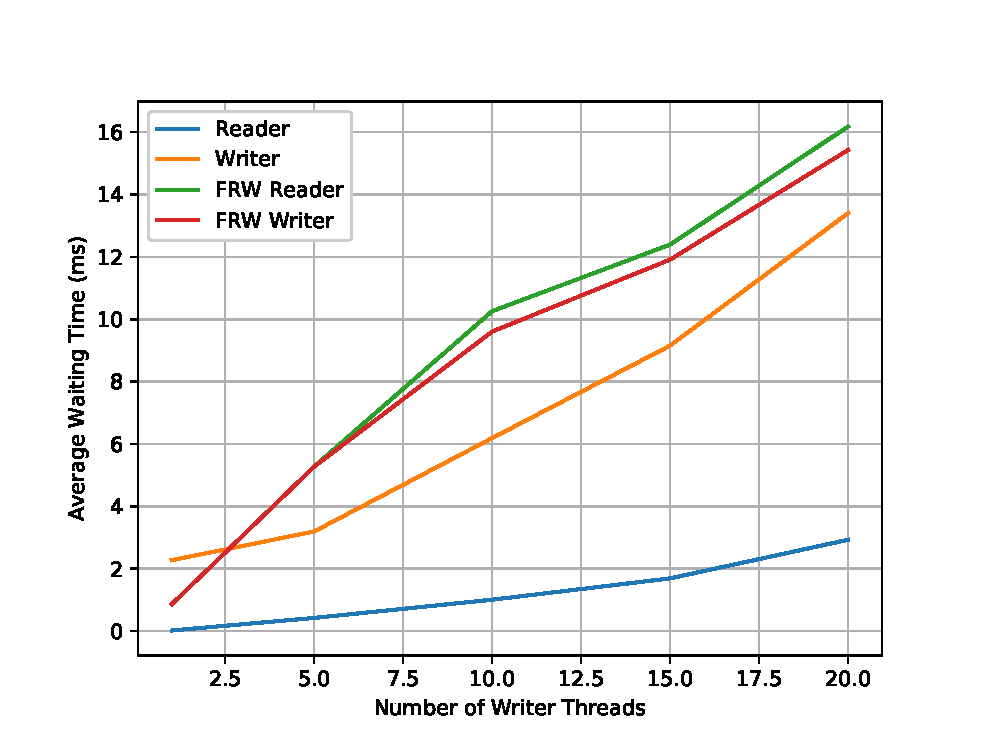
\includegraphics[scale=0.7]{./ConstantReaders-WaitingTimes.eps}
\end{center}
\begin{center}
\newpage
\begin{large}
\textbf{Worst-case Waiting Times with Constant Writers}\\
\end{large}
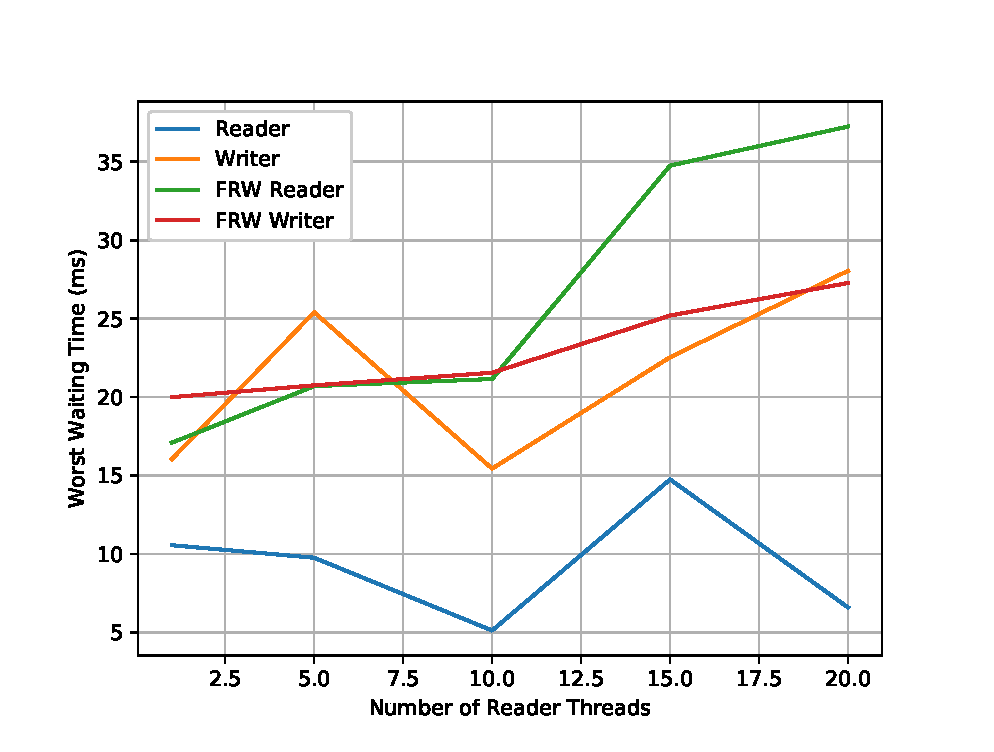
\includegraphics[scale=0.7]{./ConstantWriters-WorstTimes.eps}
\end{center}
\begin{center}
\begin{large}
\textbf{Worst-case Waiting Times with Constant Readers}\\
\end{large}
\includegraphics[scale=0.7]{./ConstantReaders-WorstTimes.eps}
\end{center}
\newpage
\section{Explaination of Results}
\begin{enumerate}
\item \textbf{Average Waiting Times With Constant Writers}\\
\begin{enumerate}
\item With increasing number of Reader threads, all the curves show an increase in the average waiting times except reader threads in normal Readers-Writers.
\item In general, the waiting times for the Fair Readers-Writers Algorithm are more than that for Readers-Writers since it has more instructions.
\item \textbf{The difference in the waiting times of the reader and writer threads for Fair Readers-Writers is almost negligible when compared to Normal Readers-Writers}, this shows the effectiveness of the FRW algorithm, and the starvation of writers in RW algorithm.
\end{enumerate}
\item \textbf{Average Waiting Times With Constant Readers}\\
\begin{enumerate}
\item This graph also tells pretty much the same story, except the fact that all the curves start off from a common low starting point, this is not unusual since we started off with a small number of writer threads and these are the threads that contribibute most to the waiting times thorugh a convoy effect.
\item Once again, the divergence in the waiting times of reader and writer threads of the normal RW algorithm is clearly visible. The writers starve more often than not.
\item The fair readers writers show a smooth increase in the waiting times but at the same time have very low difference in the waiting times of the reader and writer threads.
\end{enumerate}
\item \textbf{Worst Case Waiting Times With Constant Writers \& Readers}\\
\begin{enumerate}
\item Ideally, with increasing number of threads, the worst waiting time must also increase and this is exactly what we see in the curves of the worst waiting times.
\item We can clearly see that the worst waiting times of the writer threads from the normal RW algorithm are in the same range as the fair RW agorithm inspite of the fact that the normal RW algorithm has fewer instructions, this is an indication of starvation.
\item This is also a clear representation of the fact that neither of the threads starve when using the fair RW algorithm.
\end{enumerate}
\end{enumerate}
\end{document}